
\documentclass[conference]{IEEEtran}

\usepackage{graphicx}
\graphicspath{ {figures/} {figures/drawings/} {figures/graphs/} }

\usepackage{listings}
\def\code#1{\texttt{#1}}
\usepackage[ruled]{algorithm}
\usepackage{algpseudocode}
\usepackage{wrapfig}

%\usepackage{algorithmic}

\ifCLASSINFOpdf
\else
\fi
\hyphenation{op-tical net-works semi-conduc-tor}


\begin{document}


\title{MAM: A Memory Allocation Manager for GPUs}

\author{\IEEEauthorblockN{Can Aknesil}
        \IEEEauthorblockA{\\Computer Science and Engineering\\
                Ko\c{c} University\\
                Istanbul, Turkey\\
                caknesil13@ku.edu.tr}
	\and
	\IEEEauthorblockN{Didem Unat}
        \IEEEauthorblockA{\\Computer Science and Engineering\\
                Ko\c{c} University\\
                Istanbul, Turkey \\
		dunat@ku.edu.tr}
}


\maketitle

\begin{abstract}
Nowadays, GPUs are used in all kinds of computing fields to accelerate computer programs. We observed that allocating memory on GPUs is much slower than that of allocating memory on the CPUs. In this study, we focus on decreasing the device memory allocation overhead of GPUs. The overhead becomes significantly larger as the size of the memory segment that is being allocated increases.  In order to achieve the lowest possible overhead during device memory allocations in GPUs, we develop a thread safe memory management library called Memory Allocation Manager (MAM) for CUDA. Our library removes the allocation and the deallocation overheads occurring during the runtime, and makes the performance of CUDA programs independent from the device memory allocation size.
\end{abstract}

\begin{IEEEkeywords}
GPU, CUDA, device memory allocation, performance improvement.
\end{IEEEkeywords}


\IEEEpeerreviewmaketitle



\section{Introduction}
The current trend of computer system is to parallelize the hardware and the software programs running on it, rather than producing faster processor cores. With this trend, the usage of GPUs has been increasing in all areas of computing fields. Currently, GPUs are used for many purposes such as for graphics, machine learning, and high performance computing. Since GPUs are used extensively, it is very important to keep the performance of programs using GPUs as high as possible.

In this study, we focus on decreasing the device memory allocation overhead of GPUs. This allocation overhead is large, especially when the allocation size is large. Thus, applications requiring repetitive or large allocations may reduce the overall performance. As our measurements indicate, shown in Figure \ref{fig:m-cm}, the overhead associated to device memory allocations increases almost linearly for allocations larger than 1MB.
The similar result can be observed from a study of a group from the University of Virginia~\cite{virginia}. 

\begin{figure}[h!]
\centering
  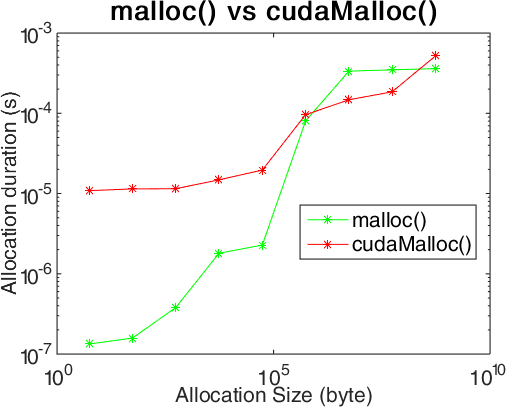
\includegraphics[width=0.8\linewidth]{malloc_vs_cuda-malloc.png}
  \caption{\code{malloc()} and \code{cudaMalloc()} durations vs allocation size}
  \label{fig:m-cm}
\end{figure}


We develop a thread safe memory management library, called Memory Allocation Manager (MAM), in order to remove the allocation overhead on GPU memory. Our library provides an abstraction layer between the programmer and the memory management module of CUDA~\cite{cuda} environment. In order to allocate and free memory using MAM, the programmer should call procedures defined in the MAM API rather than directly calling the regular \code{cudaMalloc()} and \code{cudaFree()} procedures. In this paper, we first introduce the MAM API, then its implementation. Lastly we present its performance and compare it against regular memory routines provided by CUDA. 


\section{Application Programming Interface}
%The programmer should call the memory management procedures defined in MAM API, rather than calling the regular \code{cudaMalloc()} and \code{cudaFree()} procedures after creating MAM. During the creation, a large \emph{chunk} of memory is allocated from the device memory. The details of it will be explained later.

MAM API contains five procedures that a programmer can use for memory management. 
During the creation of the MAM environment, a large \emph{chunk} of memory is allocated by MAM on the device memory, which will be explained in detail later. 

\begin{itemize} 
\item \code{MAM\_Create(maxSize)}: Creates the MAM environment. Takes a parameter that defines the size of the chunk of memory that will allocated during the creation.

\item \code{MAM\_Create\_auto()}: Creates the MAM environment. Allocates the largest possible chunk of memory during the creation.

\item \code{MAM\_Destroy()}: Destroys the MAM environment.

\item \code{MAM\_CudaMalloc(\&ptr, size)}: Allocates specified size of device memory.

\item \code{MAM\_CudaFree(ptr)}: Frees the previously allocated device memory.
\end{itemize} 

MAM can be used in three different ways:

\begin{enumerate} 
\item {By specifying the chunk size during its creation:}
\begin{lstlisting}[language=C]
MAM_Create(maxSize);
MAM_CudaMalloc(&ptr, size);
...
MAM_CudaFree(ptr);
MAM_Destroy();
\end{lstlisting}

\item {Without specifying the size of the chunk during its creation:}
In this case, the largest possible size is used. The largest possible size is allocated by performing multiple allocation operations by decreasing the allocation size exponentially starting from the size of the device memory until one of the allocations succeeds. We 
take this approach because it is not possible to allocate entire device memory. 

\begin{lstlisting}[language=C]
MAM_Create_auto();
MAM_CudaMalloc(&ptr, size);
...
MAM_CudaFree(ptr);
MAM_Destroy();
\end{lstlisting}

\item{Without explicit creation:}
In this case lazy creation occurs. \code{MAM\_Create\_auto()} is called automatically when \code{MAM\_CudaMalloc()} is first called. When all the memory allocated using MAM API is  freed, MAM automatically destroys itself.

\begin{lstlisting}[language=C]
MAM_CudaMalloc(&ptr, size);
...
MAM_CudaFree(ptr);
\end{lstlisting}
\end{enumerate} 


\section{Implementation}
During the creation of MAM, a large and continuous \emph{chunk} of memory is allocated on the device memory. The size of the chunk is expected to be equal or smaller than the maximum size of the device memory that will be used by the CUDA program at a time instance. The pointers to the segments of this large chunk of memory will be returned by MAM during the allocation process. Every object existing in MAM environment other than the \emph{chunk} live in the host memory.


\begin{figure}[h]%[23]{l}{0.18\textwidth}
\centering
  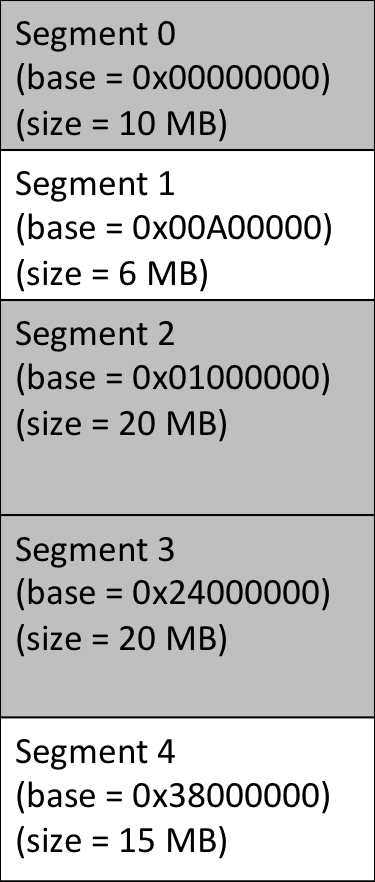
\includegraphics[width=0.18\textwidth]{random-chunk/random-chunk-pointers-and-sizes.png}
  \caption{An example of the chunk}
  \label{fig:chunk}
\end{figure}



A chunk is divided into segments that are either being used or not being used (empty) by the programmer. Figure \ref{fig:chunk} represents an example of the chunk at a time instance. The example chunk is a continuous memory and consists of 5 segments. 

In the MAM environment, each segment is represented by a \code{segment struct} instance in the host memory. The \code{segment struct} contains mainly, a pointer to the beginning of the physical segment located in the device memory, a size attribute, and a flag indicating whether it is being used by the program or not. The \code{segment struct} declaration is as follows:\\

\begin{lstlisting}[language=C]
struct segment {
	void *basePtr;
	size_t size;
	char isEmpty;
	/* attributes related to data 
	structures */
	...
};
\end{lstlisting}


\subsection{Internal Data Structures}
In MAM, there are two data structures that store the \code{segment struct} instances. The first data structure is a tree that stores all the segments. It is sorted according to the base pointer of each segment that points to the beginning of the represented physical memory. It is used when the programmer calls \code{MAM\_CudaFree(*void)} in order to find the corresponding segment using the pointer parameter.

The second data structure is a tree-dictionary that stores only the empty segments and it is sorted according to their size attribute. It is used to find an empty segment at an equal or greater size than the desired allocation size during the \code{MAM\_CudaMalloc(**void, size\_t)} call. In both data structures, a red-black tree is used since it is a balanced tree. 

\begin{figure}[h!]
\centering
  \includegraphics[width=0.8\linewidth]{pointer-tree/pointer-tree.png}
  \caption{Pointer tree}
  \label{fig:ptree}
\end{figure}

\begin{figure}
\centering
 \includegraphics[width=0.5\linewidth]{size-tree-dictionary/size-tree-dictionary.png}
  \caption{Size tree-dictionary}
  \label{fig:stree}
\end{figure}

Figure \ref{fig:ptree} and Figure \ref{fig:stree} show the corresponding data structures for the example chunk shown in Figure \ref{fig:chunk}. At that instance, there are 3 segments that are allocated by the user (Segment 0, 2, and 3), and 2 segments that are not (Segment 1, and 4). Figure \ref{fig:ptree} shows the time instance of the pointer-tree. It contains all the segments and it is sorted by the base pointers of each segment. Figure \ref{fig:stree} shows the time instance of the size-tree dictionary that contains all the empty segments. It is sorted according to the sizes of each segments. 


\section{Memory Management}
Allocation and deallocation calls to MAM API respectively starts and ends the usage of segments located in the chunk, which was previously allocated. Since the total physical memory that will be used is allocated as a large chunk during the creation of MAM environment, \code{MAM\_CudaMalloc()} and \code{MAM\_CudaFree()} calls do not actually allocate or free any physical memory but imitate the process. This is the main reason why  MAM introduces much less overhead than the CUDA memory management module. 
The initialization of the MAM environment is slow but the initialization is performed once at the beginning; once MAM is created, all the memory management calls are faster. 
Next, we will discuss the allocation and deallocation implementations in MAM. 
%The details of what happens in the MAM environment during and allocation and a deallocation is as fallows. 

\begin{figure}[!hbp]
  \centering
  \begin{minipage}[b]{0.20\textwidth}
    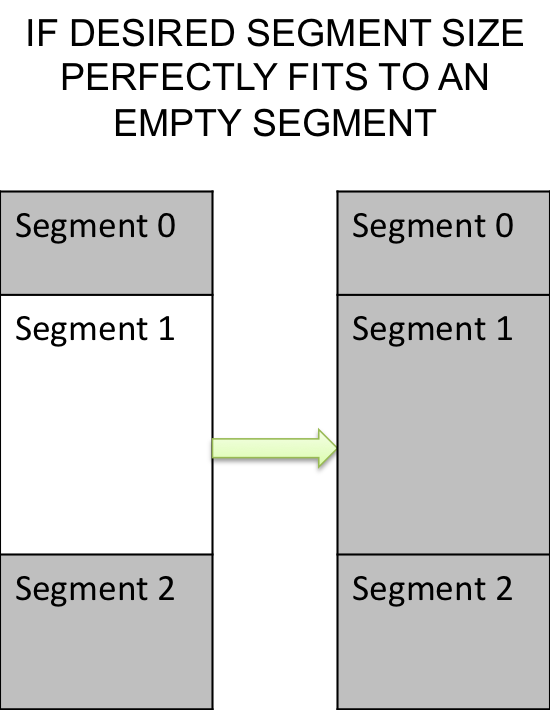
\includegraphics[width=\linewidth]{allocation/allocation1.png}
  	\caption{Allocation diagram 1}
  	\label{fig:alloc1}
  \end{minipage}
  \hspace{0.1in}
  \begin{minipage}[b]{0.20\textwidth}
    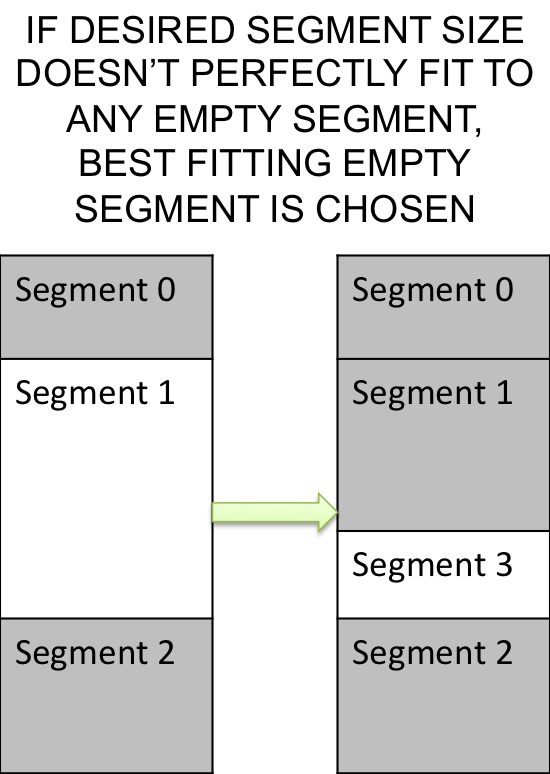
\includegraphics[width=\linewidth]{allocation/allocation2.png}
  	\caption{Allocation diagram 2}
  	\label{fig:alloc2}
  \end{minipage}
\end{figure}

\begin{algorithm}                                                                                                  
\caption{MAM Allocation Algorithm - $\mathcal{O}(\log n)$}                                                                     
\label{algorithm1}                                                                                      
\begin{algorithmic}[1] 
\Procedure{Allocate}{}      
\State Find a best-fitting empty segment from the tree-dictionary $\mathcal{O}(\log n)$
\State Mark the segment as filled $\mathcal{O}(1)$
\If {The segment perfectly fits $\mathcal{O}(1)$}
	\State {Remove segment from tree-dictionary $\mathcal{O}(\log n)$}
\Else
	\State {Resize it $\mathcal{O}(1)$}
	\State {Remove it from tree-dictionary $\mathcal{O}(\log n)$}
	\State {Create a new empty segment $\mathcal{O}(1)$}
	\State {Insert it in pointer-tree \& tree-dictionary $\mathcal{O}(\log n)$}
\EndIf
\State Return the base pointer of filled segment $\mathcal{O}(1)$
\EndProcedure
\end{algorithmic} 
\end{algorithm}

\subsection{Allocation}
When the programmer calls \code{MAM\_CudaMalloc()}, MAM searches the smallest empty segment whose size is equal or greater than the desired segment using the size tree-dictionary. If there is an empty segment with the same size, MAM marks it as filled. If the segment that is found is larger then the desired segment, a new segment that represents the non-allocated empty part is created. This procedure is illustrated in Figure \ref{fig:alloc1} and Figure \ref{fig:alloc2}. In Figure \ref{fig:alloc2}, Segment 3 is a newly created segment. 




The algorithm of MAM allocation is shown in Algorithm~\ref{algorithm1}. 
%It is the pseudo-code version of the process explained above:
The complexities of all steps in the algorithm is shown at the end of each step. The overall complexity of this allocation algorithm is $\mathcal{O}(\log n)$, where $n$ is the number of segments existing in the chunk. 

          





\subsection{Deallocation}
When the programmer calls \code{MAM\_CudaFree()}, MAM first marks the segment that is being freed as empty. Then merges the empty segment with previous and next segments if they are also empty. This procedure is illustrated in Figure \ref{fig:dealloc}. % and the algorithm for MAM deallocation is 

The algorithm of MAM deallocation is shown in Algorithm~\ref{algorithm2}. The overall completely of the deallocation algorithm is also $\mathcal{O}(\log n)$, where n is the number of the segments in the chunk. 
%shown in Algorithm 2. 


\begin{figure}[h!]
\centering
  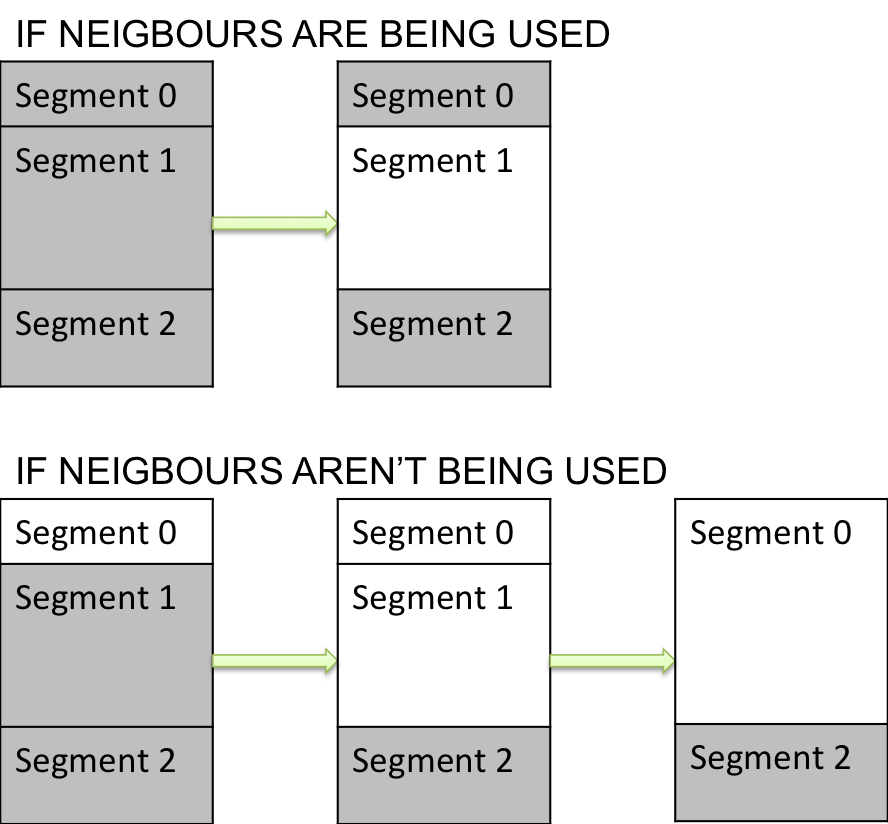
\includegraphics[width=0.75\linewidth]{deallocation/deallocation.png}
  \caption{Deallocation diagram}
  \label{fig:dealloc}
\end{figure}




\begin{algorithm}                                                                                                  
\caption{MAM Deallocation Algorithm - $\mathcal{O}(\log n)$}                                                                     
\label{algorithm2}                                                                                      
\begin{algorithmic}[1] 
\Procedure{Deallocate}{}      
\State Find the segment in the pointer-tree $\mathcal{O}(\log n)$
\State Mark the segment as empty $\mathcal{O}(1)$
\State Get previous and next segments $\mathcal{O}(\log n)$
\If {the previous segment is empty $\mathcal{O}(1)$}
	\State {Remove the segment being newly emptied from pointer-tree and tree-dictionary $\mathcal{O}(\log n)$}
	\State {Destroy the segment being newly emptied $\mathcal{O}(1)$}	
	\State {Resize previous segment $\mathcal{O}(1)$}
	\State {Replace it in tree-dictionary $\mathcal{O}(\log n)$}
	\State {Assign it to the variable stored the destroyed segment $\mathcal{O}(\log n)$}
\EndIf
%\If {The next segment is empty $\mathcal{O}(1)$}
	\State //repeat the similar procedure for next segment. 
%\EndIf
\EndProcedure
\end{algorithmic} 
\end{algorithm}




The allocation and deallocation algorithms are used in the implementation of MAM API, respectively in the procedures \code{MAM\_CudaMalloc()} and \code{MAM\_CudaFree()}. Thus, the complexities of both allocation and deallocation are $\mathcal{O}(\log n)$ in terms of the number of segments.


\section{Performance Evaluation}
We demonstrate the performance of MAM in two ways: 
in terms of the allocation size, and in terms of the number of previously allocated segments.
We used Tesla K20m as the GPU testbed, Linux 2.6.32-431.11.2.el6.x86\_64 as the kernel and NVCC 7.0, V7.0.27 as CUDA Compilation Tools in all of our tests.

In order to measure the performance in terms of allocation size, 
we created a histogram that stores the time elapsed during allocation 
for different allocation sizes from 1Byte to 1GigaByte.
% in 9 subintervals divided
% logarithmically). 
We filled the histogram by allocating the device memory 
 parts of random sizes over and over again until there is no more space. 

Figure \ref{fig:cm-mcm} and Figure \ref{fig:cf-mcf} show the performance comparison between regular \code{cudaMalloc()} and \code{MAM\_CudaMalloc()}, and \code{cudaFree()} and \code{MAM\_CudaFree()}, respectively, in terms of allocation size.

\begin{figure}[h!]
\centering
  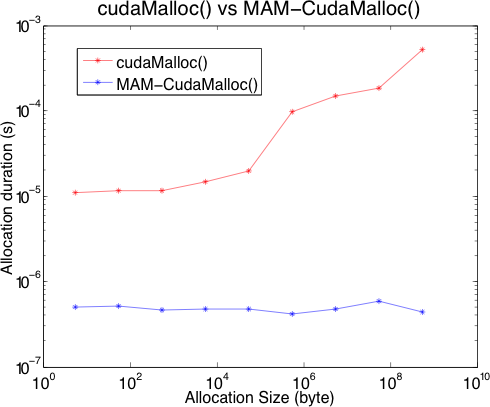
\includegraphics[width=0.85\linewidth]{cudamalloc-vs-mamcudamalloc.png}
  \caption{\code{cudaMalloc()} vs \code{MAM\_CudaMalloc()} comparison}
  \label{fig:cm-mcm}
\end{figure}

\begin{figure}[h!]
\centering
  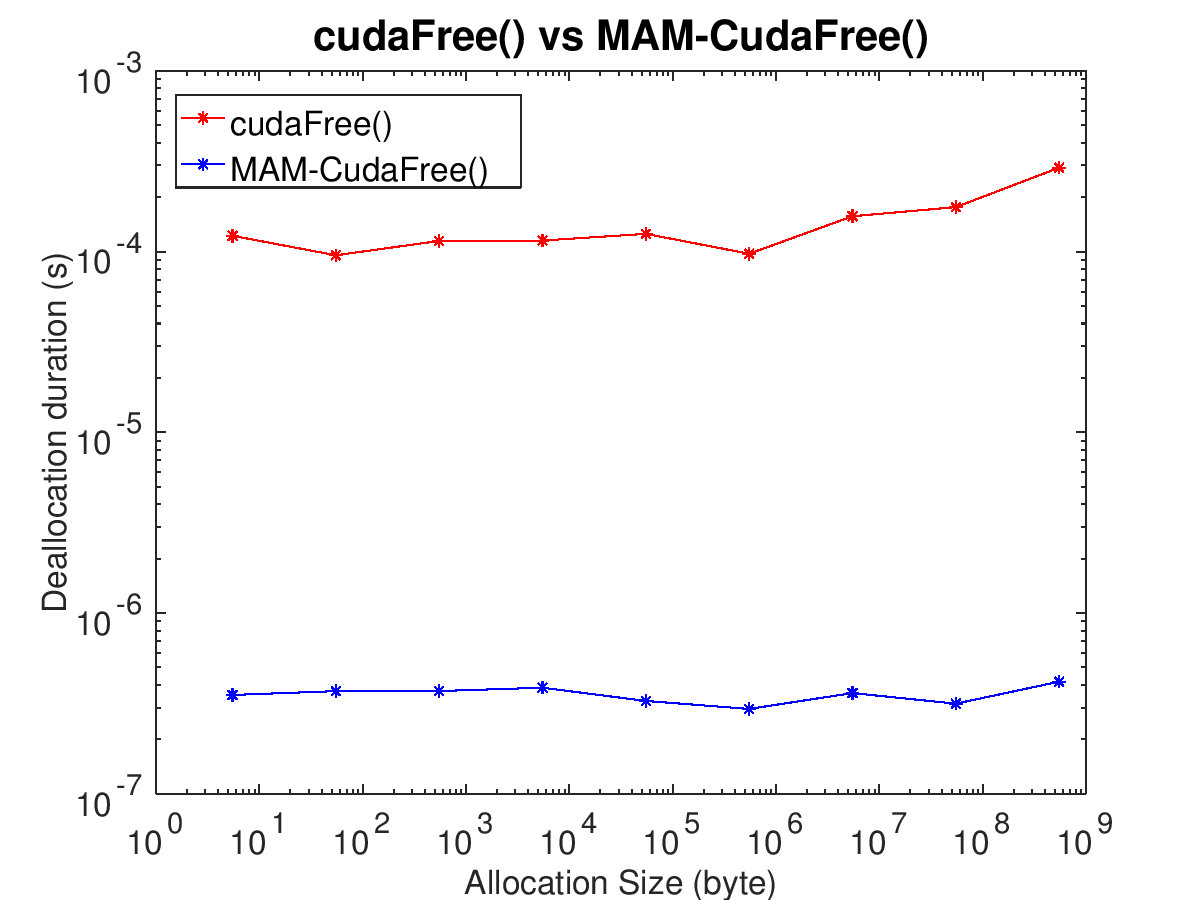
\includegraphics[width=\linewidth]{cudafree-vs-mamcudafree.png}
  \caption{\code{cudaFree()} vs \code{MAM\_CudaFree()} comparison}
  \label{fig:cf-mcf}
\end{figure}

As shown in these figures, while allocation duration of \code{cudaMalloc()} increases swiftly, the duration of \code{MAM\_CudaMalloc()} stays almost constant. MAM removes the allocation and deallocation overhead and makes the performance of allocations independent from the allocation size. This result was expected because MAM moves the entire physical memory allocation overhead to the creation of MAM environment from individual allocations. Even though the initialization of MAM is slow, once it is initialized, there is no significant overhead caused by memory allocations or deallocations. Because, there is no physical memory allocation after the creation of MAM and the allocation size has no effect on the complexity of MAM.
% it is meaningless to measure the performance according to the allocation size. 

The second performance measurement is based on the total number of existing segments during allocation or deallocation. This is meaningful because the size of data structures used in the MAM environment increases with the number of segments. 
%This measurement is according to the number of previously allocated segments. 
In order to measure the performance in terms of the number of previously allocated segments, we measured the time elapsed during the first allocation after allocated variable number of segments. In this measurement, the allocation size was random between 1Byte to 10Bytes, sufficiently small so that we could make large number of allocations up to $10^7$ before the device memory is full. Figure \ref{fig:cm-mcm-pa} shows the performance comparison between regular \code{cudaMalloc()} and \code{MAM\_CudaMalloc()} in terms of the number of previously allocated segments. 

\begin{figure}[h!]
\centering
  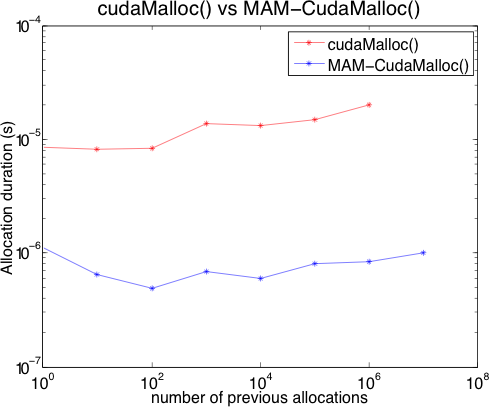
\includegraphics[width=0.8\linewidth]{cudamalloc-vs-mamcudamalloc-pa.png}
  \caption{\code{cudaMalloc()} vs \code{MAM\_CudaMalloc()} comparison according to number of previous allocations}
  \label{fig:cm-mcm-pa}
\end{figure}

According to this performance measurement, MAM is faster than CUDA and the duration of MAM allocation increases more slowly than actual CUDA allocation for the number of previously allocated segments larger than 100. This is the result of the fact that allocation algorithm of MAM is $\mathcal{O}(\log n)$, since the red-black tree used in MAM environment is a balanced tree. 

We should also mention that when the programmer makes a very large number of small device memory allocations, MAM uses lots of host memory, since a \code{segment struct} instance is created for each segment.



\section{Discussion \& Related Work}
This study only covers the performance comparison of MAM with CUDA device memory management. However, MAM is completely applicable to any other environment that involves allocation and deallocation of a contiguous space of any kind, such as pinned memory allocation of CUDA~\cite{ICPP-Burak} or host memory allocation. MAM will work exactly the same way with any of these environments since it does not depend on the actual, or physical allocation procedure once it is created.

In the literature, there is a group that also focusses on GPU memory alloation and deallocation overhead \cite{regeff}. They compare current GPU memory allocators and propse a new one that is register efficient. There are a lot of studies~\cite{ICPP-Burak, dCUDA, CuMAS} about GPU memory management, mainly  focusing 
on reducing data transfer overhead between the host and device memory. A study deals with the effective usage of relatively small GPU memory by using it as a cache for the host memory and transferring data between the two memories during runtime \cite{gpudmm}. A second study that also focuses on small device memory size decreases data transfer overhead between device and host memory by directly connecting  a Solid State Disk (SSD) to a GPU \cite{gpussd}. A group has developed a tool to manage device memory so that multiple applications can use the GPU without any problems \cite{gdm}. Another study integrated GPU as a first-class resource to the operating system \cite{gdev}. 

To our knowledge, there is no study focusing specifically on solving GPU memory allocation overhead. Programmers generally write their own memory manager for their specific application when it is needed. MAM offers a generalized solution, is independent of an applications, and provides efficient data structures to keep the overhead low. 
% to all kind of allocation overhead problems.


\section{Conclusion}
In this study, we focused on reducing the memory allocation overhead in GPUs and we developed MAM, which is a library for CUDA. This library abstracts the CUDA memory management module from the program and succeeds to remove the overhead by moving all the overhead to the beginning of the program. MAM currently offers a solution for the memory allocation problem of CUDA but it can be easily extended to be used in other platforms. Our future work will extend this work to Intel Xeon Phi architectures and other GPU programming models. 
%solve other allocations overhead problem.


\begin{thebibliography}{1}

\bibitem{cuda}
''CUDA Toolkit'', NVIDIA Developer, 2017. \lbrack Online\rbrack . Available: https://developer.nvidia.com/cuda-toolkit. \lbrack Accessed: 10- Jul- 2017\rbrack .


\bibitem{virginia}
CUDA Memory Management Overhead. \lbrack Online\rbrack . Available: https://www.cs.virginia.edu/~mwb7w/cuda\_support/memory\_management\_overhead.html. \lbrack Accessed: 14-Oct-2016\rbrack .

\bibitem{gpudmm}
Y. Kim, J. Lee, and J. Kim, ''GPUdmm: A high-performance and memoryoblivious
GPU architecture using dynamic memory management,'' in
Proc. IEEE Int. Symp. High Perform. Comput. Archit. (HPCA), Feb. 2014,
pp. 546-557.

\bibitem{gpussd}
J. Zhang, D. Donofrio, J. Shalf, M. Kandemir, and M. Jung. Nvmmu:
A non-volatile memory management unit for heterogeneous gpu-ssd
architectures. PACT 2015, 2015.

\bibitem{gdm}
K. Wang, X. Ding, R. Lee, S. Kato, and X. Zhang, ''Gdm:
Device memory management for gpgpu computing,'' in The
2014 ACM International Conference on Measurement and
Modeling of Computer Systems, SIGMETRICS, (New
York, NY, USA), pp. 533-545, ACM, 2014.

\bibitem{gdev}
S. Kato, M. McThrow, C. Maltzahn, and S. A. Brandt. Gdev:
First-class gpu resource management in the operating system.
In USENIX Annual Technical Conference, 2012.

\bibitem{ICPP-Burak}
B. Bastem, D. Unat, W. Zhang, A. Almgren, and J. Shalf. 
Overlapping Data Transfers with Computation on GPU with Tiles, 
The 46th International Conference on Parallel Processing, ICPP 2017

\bibitem{CuMAS}
Mehmet E. Belviranli, Farzad Khorasani, Laxmi N. Bhuyan, and Rajiv Gupta. 2016. CuMAS: Data Transfer Aware Multi-Application Scheduling for Shared GPUs. In Proceedings of the 2016 International Conference on Supercomputing (ICS '16). ACM, New York, NY, USA, Article 31, 12 pages. 

\bibitem{dCUDA}
T. Gysi, J. Bar and T. Hoefler, 
dCUDA: Hardware Supported Overlap of Computation and Communication, 
SC16: International Conference for High Performance Computing, Networking, Storage and Analysis, Salt Lake City, UT, 2016, pp. 609-620.

\bibitem{regeff}
M. Vinkler and V. Havran, "Register Efficient Dynamic Memory Allocator for GPUs", Computer Graphics Forum, vol. 34, no. 8, pp. 143-154, 2015.

\end{thebibliography}





\end{document}


